\documentclass[10pt]{article}
\usepackage[polish]{babel}
\usepackage[utf8]{inputenc}
\usepackage[T1]{fontenc}
\usepackage{amsmath}
\usepackage{amsfonts}
\usepackage{amssymb}
\usepackage[version=4]{mhchem}
\usepackage{stmaryrd}
\usepackage{graphicx}
\usepackage[export]{adjustbox}
\graphicspath{ {./images/} }
\usepackage{hyperref}
\hypersetup{colorlinks=true, linkcolor=blue, filecolor=magenta, urlcolor=cyan,}
\urlstyle{same}

\title{KLASY PIERWSZE I DRUGIE }

\author{}
\date{}


\begin{document}
\maketitle
\begin{enumerate}
  \item Każda z liczb \(x_{1}, x_{2}, \ldots, x_{101}\) jest równa 1 lub -1 . Wyznacz najmniejszą możliwą wartość wyrażenia
\end{enumerate}

\[
x_{1} x_{2}+x_{2} x_{3}+x_{3} x_{4}+\cdots+x_{101} x_{1}
\]

\begin{enumerate}
  \setcounter{enumi}{1}
  \item Która z liczb jest większa \(3^{100}-2^{150}\) czy \(3^{50}-2^{75}\) ? Odpowiedź uzasadnij.
  \item Czworokąt \(A B C D\) jest kwadratem. Wyznacz długość odcinka \(E C\), jeśli \(|A F|=4 \mathrm{i}|F B|=3 \mathrm{i}\) kąt \(A F E\) jest kątem prostym.\\
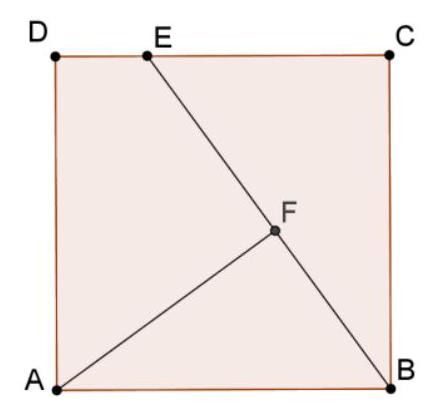
\includegraphics[max width=\textwidth, center]{2024_11_21_cb743ddb4cacb96e214dg-1(1)}
\end{enumerate}

\section*{KLASY TRZECIE}
\begin{enumerate}
  \item Rozwiąż układ równań w liczbach całkowitych nieujemnych.
\end{enumerate}

\[
\left\{\begin{array}{l}
a+b c=3 b \\
b+c a=3 c \\
c+a b=3 a
\end{array}\right.
\]

\begin{enumerate}
  \setcounter{enumi}{1}
  \item Udowodnić, że jeśli \(a+b+c=0\) to \(a^{3}+b^{3}+c^{3}=3 a b c\).
  \item \(W\) trójkącie \(A B C\) punkt \(H\) jest ortocentrum, punkt \(D\) spodkiem wysokości CD, punkt E środkiem boku AC a punkt F środkiem odcinka BH. Udowodnij, że kąt EDF jest prosty..\\
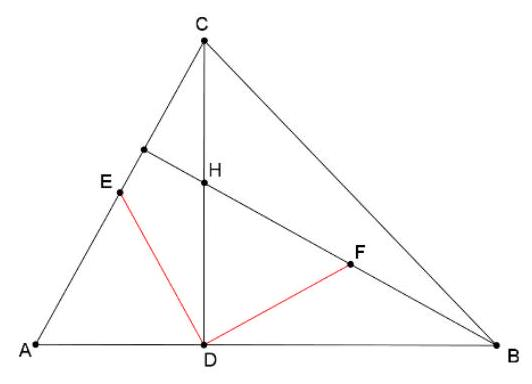
\includegraphics[max width=\textwidth, center]{2024_11_21_cb743ddb4cacb96e214dg-1}
\end{enumerate}

Rozwiqzania należy oddać p. Jarostawowi Szczepaniakowi do piatku 10 czerwca do godziny 15.00 lub przestać na adres \href{mailto:jareksz@interia.pl}{jareksz@interia.pl} do soboty 11 czerwca do pótnocy.


\end{document}